% !TEX encoding = UTF-8 Unicode
%% Erläuterungen zu den Befehlen erfolgen unter
%% diesem Beispiel.
\documentclass{scrartcl}
\usepackage[utf8]{inputenc}
\usepackage[T1]{fontenc}
\usepackage[ngerman]{babel}
\usepackage{graphicx}
\usepackage{listings}

\newcommand{\funktion}[1]{\emph{#1}}



\title{Entwicklung eines graphischen Editors für die Audiosignalverarbeitung durch VST-Plugins}
\author{Johannes Unger}
\date{\today}
\begin{document}
\maketitle
\newpage
\tableofcontents
% !TEX encoding = UTF-8 Unicode
\section{Einleitung}
\subsection{Motivation}
\begin{figure}[htbp]
	\centering
 	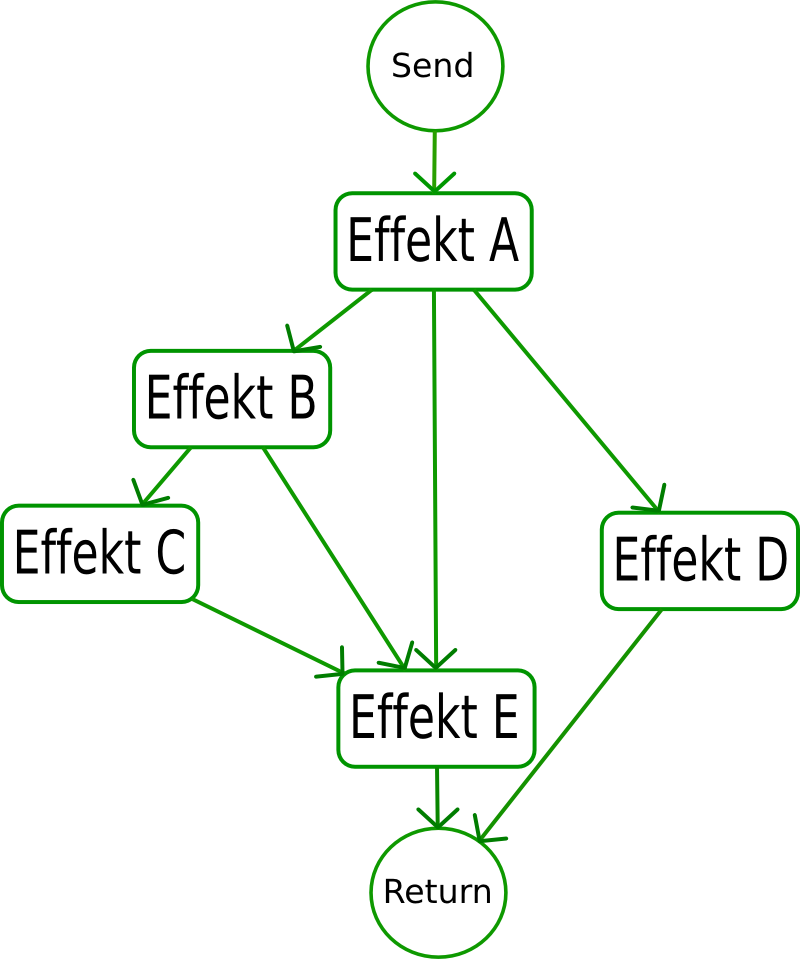
\includegraphics[scale=0.12]{../graphics/free_order}
	\caption{Beispiel einer Effektverkettung, wie sie in der Realität möglich wäre}
	\label{freeOrder}
\end{figure}
Moderne DAWs\footnote{Digital Audio Workstation: computergestütztes System für Tonaufnahme, Musikproduktion, Abmischung und Mastering} bieten umfangreiche und kreative Werkzeuge zum Erzeugen und Manipulieren von Klangereignissen. In vielen Fällen orientierten sich solche Programme anhand real existierender Hardware. So wird oftmals ein Klangereignis einem Kanal in einem virtuellen Mischpult zugeordnet, der einem real existierenden Gerät nachempfunden wurde.
\\\\
Es können neben der Lautstärkeregelung und Stereoverteilung auch Effekte in einen solchen Kanal eingeschliffen werden. Hier unterscheiden sich allerdings die Möglichkeiten zwischen real existierender Hardware und der Software Lösung. Während es in der Realität unzählige Möglichkeiten gibt verschiedene Effekte zu kombinieren - sprich zu „verdrahten“ (siehe Abbildung \ref{freeOrder}) - sind die meisten DAWs in ihren Möglichkeiten beschränkt.
Dies soll anhand des Sequenzers ''Cubase\footnote{verwendete Version: Cubase SL 2.0 ( http://www.steinberg.net )}'' veranschaulicht werden:
\\\\
\begin{figure}[htbp]
	\centering
	\begin{minipage}[b]{7.2 cm}
		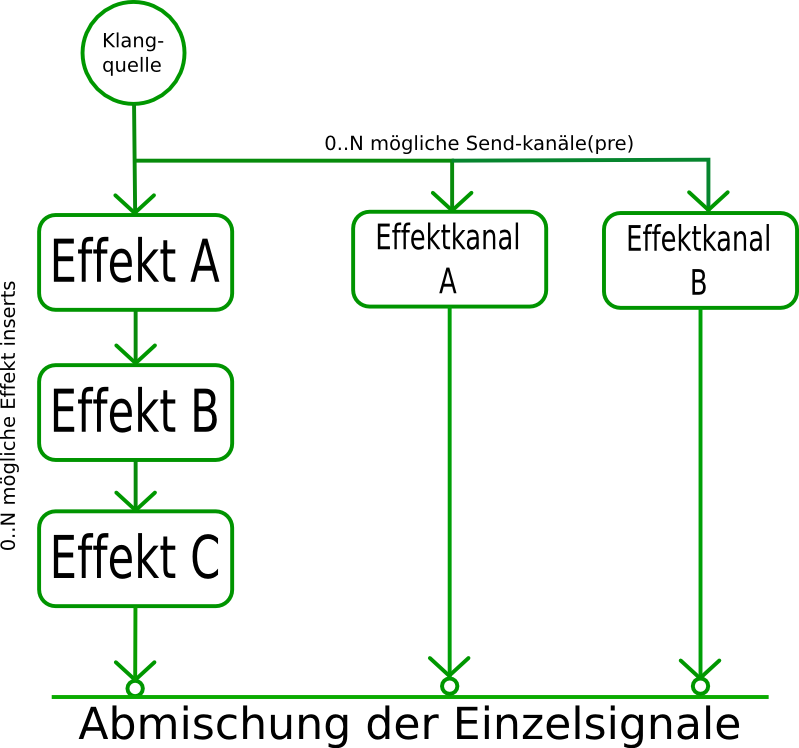
\includegraphics[scale=0.15]{../graphics/send-pre}
	\end{minipage}
	\begin{minipage}[b]{7.2 cm}
 		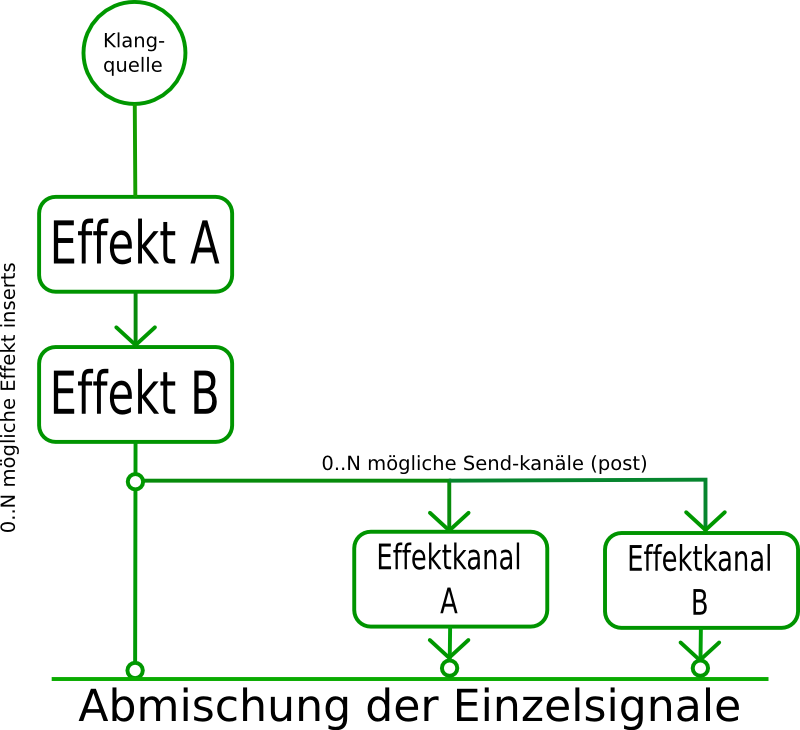
\includegraphics[scale=0.15]{../graphics/send-post}
	\end{minipage}
	\caption{Effektkette mit 'send' Abzweigung, jeweils als 'pre' und als 'post' Variante (v.l.n.r)}
	\label{send}
\end{figure}
Jede Klangquelle in Cubase, sei es eine Audiospur oder ein virtuelles Instrument, wird einem eigenen Kanal in dem virtuellen Mischpult zugeordnet. 
Jeder Kanal hat neben einem Equalizer und einer Pan-/Lautstärkeregelung eine feste Anzahl von  ''Insert-Slots''. In einen solchen ''Slot'' kann genau ein Effektmodul geladen werden (in Abbildung 2 und 3 als ''Effekt A..X'' bezeichnet). Jeder dieser Effekte wird nacheinander durchlaufen, was einer Reihenschaltung entspricht. Für eine Parallelschaltung steht eine begrenzte Anzahl von sogenannten ''Send'' Signalwegen zur Verfügung, von denen es zwei Varianten gibt: ''pre-send'' und ''post-send'' (siehe Abbildung \ref{send}).
Je nach Typ wird das Audiosignal vor der Insert-Effektkette abgegriffen oder danach und in einen Effekt Kanal geleitet. Dieser Effektkanal besteht wiederum aus einer begrenzten Anzahl aus ''Insert-Slots''.
\\\\
Diese Möglichkeiten sind für die meisten Produktionen vollkommen ausreichend, da der Unterschied - ob ein Effekt in Reihe oder parallel geschaltet wurde - abhängig vom Effekttyp - meistens sehr gering ist. Dennoch ist es manchmal wünschenswert etwas mehr Kontrolle und Übersicht über die Zusammensetzung der einzelnen Signalwege zu haben. 
\\\\
\begin{figure}[htbp]
	\centering
	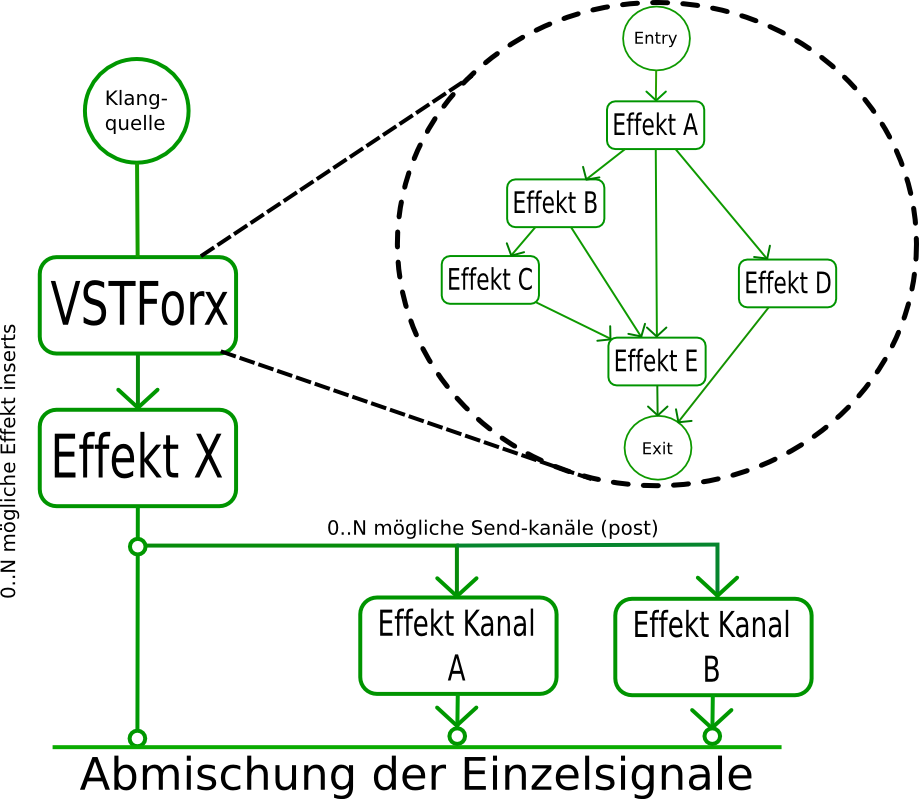
\includegraphics[scale=0.2]{../graphics/solution_vstforx}
 	\caption{Die Idee - freie Verdrahtung als Effekt}
	\label{solutionVSTForx}
\end{figure}
Ziel ist es ein Programm zu entwickeln, das genau das bietet. Es sollte es möglich machen beliebig viele Effekte auf eine virtuelle ''Bühne'' zu laden um diese wiederum beliebig ''verdrahten'' zu können. Das Programm sollte selbst ein Effekt sein. Somit wäre die Integration in eine DAW Umgebung denkbar einfach (siehe Abbildung \ref{solutionVSTForx}).\\
Die meisten Effekte werden durch Parameter gesteuert. Diese Parameter sollten sich ebenfalls in Form von Reglern auf die ''Bühne'' holen und von dort aus bedienen lassen. 
Diese Regler könnte man verbinden und somit mehrere Regler mit einmal steuern. So wäre es zum Beispiel möglich die Intensität eines Halleffektes und die Intensität eines Verzerrers mit einem einzigen Regler gleichzeitig zu steuern.
Darüber hinaus bietet es sich an den Signalfluss und das verhalten der Effekte durch zusätzliche Module manipulierbar beziehungsweise erweiterbar zu machen. Es wäre zum Beispiel eine Art ''Step-Sequencer'' denkbar. Ein Modul welches Rhythmisch zwischen verschiedenen Signalwegen umschaltet. 
\\\\
Das Programm wäre ein ideales Werkzeug zum erschaffen von kreativen Klangexperimenten.
\subsection{Der Name}
Als Programmname entschied ich mich für ''VSTForx''. 
\paragraph{VST} VST\footnote{Abkürzung für ''Virtual Studio Technology'' - Steinberg Media Technologies GmbH} ist eine Plugin-Schnittstelle im Bereich Audioverarbeitung. Aufgrund der hohen Verbreitung von VST-Plugins, wird die zu entwickelnde Software diese Schnittstelle Hauptsächlich unterstützen.
\paragraph{Forx} ein Kunstwort das vom englischen Wort ''fork'' abgeleitet ist. Fork bedeutet Gabelung oder Abzweigung und beschreibt somit ziemlich treffend den Hauptzweck der Software.
% !TEX encoding = UTF-8 Unicode
\section{Anforderungen}
\subsection{VST}
Da VSTForx ein VST-Plugin werden soll muss es natürlich den Schnittstellen des VST Standards entsprechen. Es stehen hierbei zwei Versionen zur Auswahl: VST2.x und VST3.x.
\paragraph{VST2.x}
Das VST2.x SDK hatte im Jahre 2006 sein letztes Update erfahren(\cite{stein06}). Seine Ursprünge reichen bis in das Jahr 1990 zurück als die VST Schnittstelle entwickelt wurde.
Da in den 90er Jahren die Rechenleistung begrenzt war, war ein wesentliches Entwurfsziel die Performance. So ist ein Großteil des SDKs ist in C geschrieben \footnote{es existieren aber - um die Implementierung zu vereinfachen - C++ Wrapperklassen.}.
Aus heutiger Sicht können viele in der VST2.x SDK verwendete Techniken als veraltet betrachtet werden. So wird zum Beispiel zur 'Host nach Plugin Kommunikation' lediglich eine Methode verwendet die über sogenannte Opcodes\footnote{Abkürzung für Operation Code. Jede aufrufbare Operation wird durch einen Code Symbolisiert und als Parameter übergeben.} parametrisiert werden. Es werden sehr häufig '*void' Zeiger benutzt was zusammen mit einer schlechten Dokumentation schnell zu schwer auffindbaren Fehlern führen kann. 
\paragraph{VST3.x}
Das VST3.x SDK wurde im Jahre 2008 eingeführt und ist eine vollständige Neuentwicklung\cite{stein08}.Es ist komplett Objekt orientiert und bietet dem Entwickler eine Reihe an neuen Features die, die Entwicklung von VST-Plugins vereinfachen. 
\\\\
Obwohl aus rein technischer Sicht die Entwicklung eines VST3.x-Plugins lukrativer wäre, viel die Wahl dennoch auf die VST2.x Version. VST2.x-Plugins sind weiter verbreitet und werden von fast allen DAWs unterstützt.
Ein VST-Plugin tritt in der Form einer Dynamisch ladbaren Bibliothek auf. Je nach System ist es unter Windows eine ''.dll'' Datei oder unter Mac OSX ein sogenanntes ''Ressource Bundle''.

\subsection{Alternative Schnitstellen}
% !TEX encoding = UTF-8 Unicode
\section{Fachliches Umfeld}
\subsection{Der Sampleblock}
Ein digitales Audiosignal besteht aus einer Menge einzelner Werte, den Samples. Der Sampleblock stellt die Menge an Samples dar, die von einem VST-Plugin auf einmal bearbeitet werden kann. Die Größe des Sampleblockes ist Ausschlaggebend für die Performance und die Latenz\footnote{die Verzögerung zwischen Signalein- und ausgabe.} einer DAW Umgebung. Je niedriger die Blockgröße desto niedriger die Latenz, desto höher die CPU Auslastung.
\subsection{\label{Prozess}Der Prozess}
In der Terminologie des VST-SDK, ist mit Prozess der Teil eines Plugins gemeint, der für die Bearbeitung aller Pluginein- und ausgänge verantwortlich ist.
\\\\
Im VST2.x SDK ist dies eine Methode namens ''processReplacing''. Ihr werden als Parameter die Eingangs- und ausgangssampleblöcke übergeben. Die Anzahl der Sampleblöcke ist abhängig von der Anzahl der Pluginein- sowie ausgangskanäle. So werden zum Beispiel einem Stereoplugin zwei Eingangsampleblöcke übergeben, jeweils ein Block für ''Rechts'' und ein Block für ''Links''.
\\\\
Der Ablauf eines Prozesses kann wie folgt Skizziert werden:
\begin{itemize}
	\item die DAW füllt die Plugin-Eingangssampleblöcke mit den Daten eines Audiokanals
	\item die DAW ruft die ''processReplacing'' Methode des Plugins auf.
	\item das Plugin verarbeitet die Eingangssampleblöcke und schreibt die Ergebnisse in die entsprechenden Ausgangssampleblöcke
	\item die DAW verarbeitet die Ausgangssampleblöcke weiter
\end{itemize}
Dieser Vorgang wird, während eine DAW im ''Abspielmodus'', ist ständig wiederholt.

% !TEX encoding = UTF-8 Unicode 
\section{Ausgewählte Problemstellungen}
%%%%%%
\subsection{Die Effektverkettung}
\paragraph{Das Modell}
VSTForx soll Plugins laden und mittels ''virtueller'' Kabel verbinden können. Als mathematisches Modell ist für diese Aufgabe der gerichtete Graph geeignet. Die Knoten repräsentieren die Plugins und die Kanten die Verbindungen.
\paragraph{Die Berechnungsreihenfolge}
Wie bereits in Kapitel \ref{Prozess} beschrieben erzeugt ein Plugin seine Ausgabe anhand einer ''processReplace'' Methode. Das Programm muss nun den beschriebenen Prozessablauf mit den geladenen Plugins durchführen. Doch in welcher Reihenfolge sollten diese Aufrufe stattfinden?\\\\
\begin{figure}[h]
	\centering
 	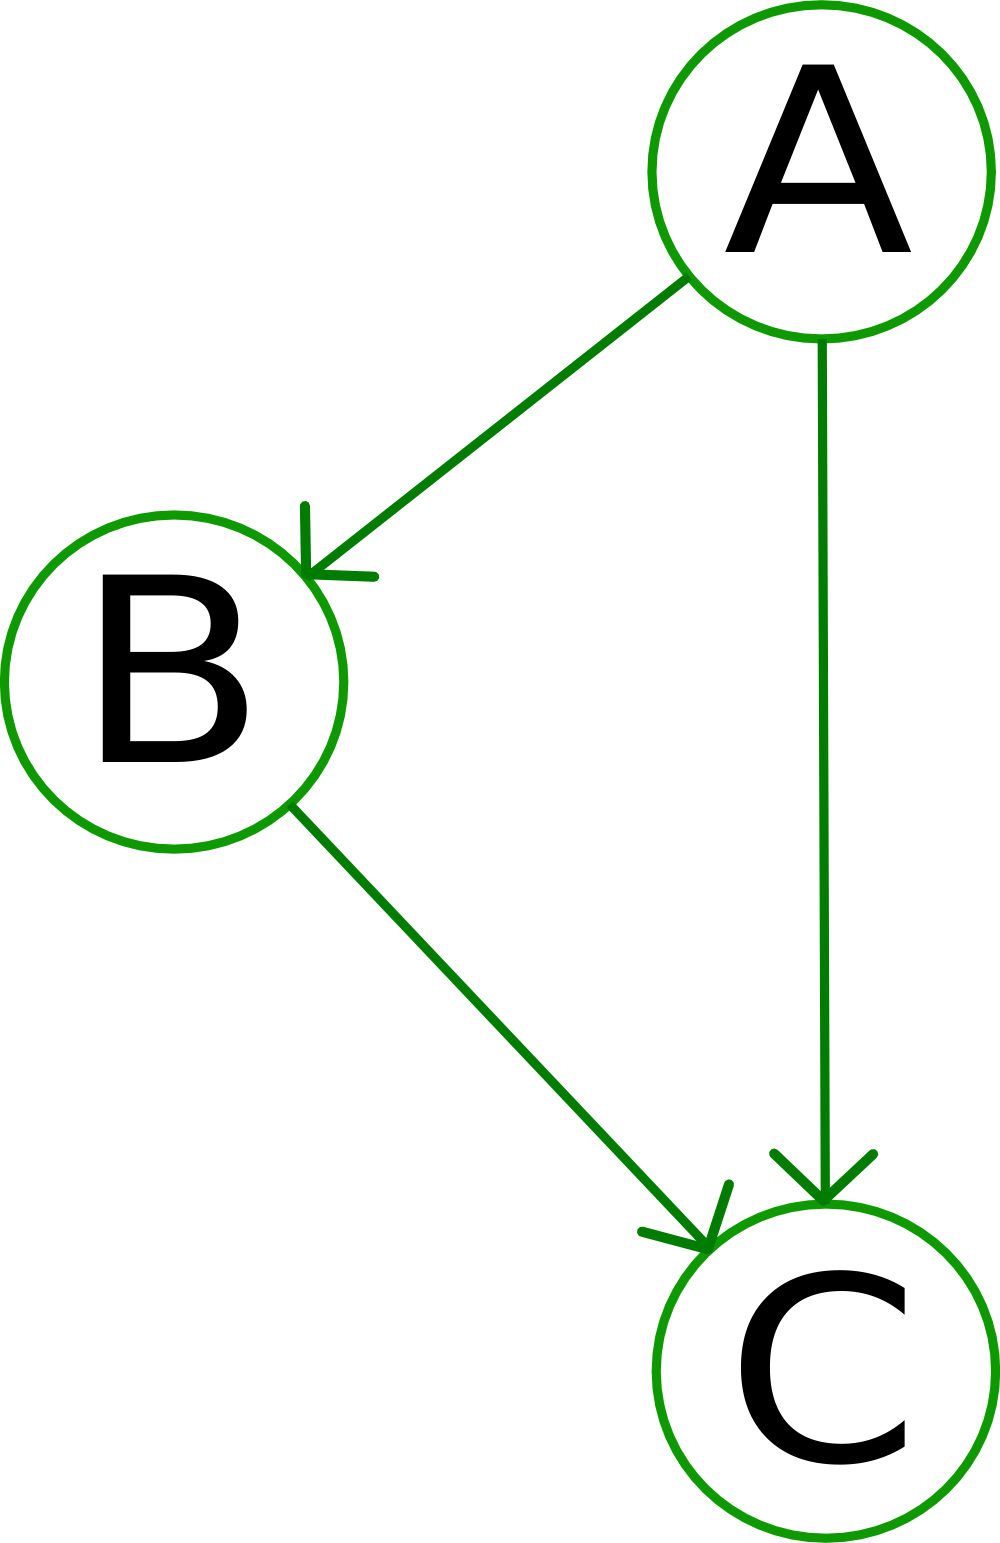
\includegraphics[scale=0.1]{../graphics/g01.png}
	\caption{Beispiel eines Plugin Graphen}
	\label{g01}
\end{figure}
Gegeben sei folgendes Beispiel:
\\\\
Jeder Knoten entspricht einem Plugin (A-C). Eine gerichtete Kante entspricht einer Verbindung von Pluginausgang zu Plugineingang.
\\\\
Der erforderliche Prozessablauf für Abbildung \ref{g01} wäre:
\begin{enumerate}
	\item bereite Inputsampleblöcke für Plugin-A vor
	\item führe ''processReplace'' mit Plugin-A aus
	\item bereite Inputsampleblöcke für Plugin-B vor (mit der Ausgabe von Plugin-A)
	\item führe ''processReplace'' mit Plugin-B aus
	\item\label{PlugC}bereite Inputsampleblöcke für Plugin-C vor (mit der Ausgabe von Plugin-A und B)
	\item führe ''processReplace'' mit Plugin-C aus
	\item übertrage die Ausgabe von Plugin-C in die Programm(VSTForx) Ausgabesampleblöcke
\end{enumerate}
Wie in Schritt \ref{PlugC} zu sehen ist zur korrekten Ausführung von Plugin-C notwendig, dass die Plugins A und C bereits bearbeitet wurden. Das bedeutet: Plugin-C ist von Plugin-A und Plugin-B abhängig. \\\\
In der Graphentheorie gibt es einen Algorithmus der in der Lage ist Abhängigkeiten aufzulösen: Die Topologische Sortierung.
\\\\
Die Topologische Sortierung basiert auf der Durchlaufstrategie Tiefensuche\footnote{oder auch DFS - engl.: Depth First Search}. \\
''Sie erzeugt eine lineare Anordnung von Knoten eines Graphen. Existiert eine Kante zwischen den Knoten (u, v),  so wird u vor v geordnet."\cite{bgl01}\\
Das Resultat der Topologischen Sortierung ist daher eine sortierte Menge an Knoten deren Reihenfolge  genau ihren Abhängigkeiten entspricht.
In unsrem Beispiel würde die Topologische Sortierung die (Plugin-)Knotenmenge \{A, B, C\}\footnote{vorausgesetzt Knoten A ist der Startknoten der Topologischen Sortierung} ergeben.
\paragraph{Rückkopplungen}
Eine Einschränkung der Topologischen Sortierung ist es, dass die zu sortierenden Graphen keine Zykel enthalten dürfen. Dies hat für VSTForx zur Auswirkung dass keine Rückkopplungen ''geschaltet'' werden können. Eine Rückkopplung wäre es zum Beispiel, wenn der Ausgang eines Plugins, direkt oder über Umwege, wieder an seinem Eingang liegen würde. Sollten Rückkopplungsschaltungen unterstützt werden, könnte man die betreffenden Knoten lokalisieren und in einen Subgraphen substituieren. Dieser Subgraph könnte dann die Knoten durch einen alternativen Algorithmus, einen der Rückkopplungen unterstützt, behandeln. Dies ist jedoch nicht vorgesehen. \\
Die Topologischen Sortierung ist es allerdings in der Lage zu erkennen ob ein Graph Zyklisch ist. Zur Vermeidung von Fehlverhalten werden daher Zyklische Graphen nicht zugelassen.  
\paragraph{Inaktive Knoten}
%%%%%%
\subsection{Das Latenzproblem}
%%%%%%
\subsection{Persistenz}
%%%%%%
\subsection{Portabilität}
%%%%%%
\subsection{Nebenläufigkeit}
%%%%%%
\subsection{Verwendung von Speicherdateien auf unterschiedlichen Systemen}
%\include{kap_Anforderungsdefinition}
% !TEX encoding = UTF-8 Unicode
\section{Systementwurf}
\subsection{Grundstruktur}
\begin{figure}[htbp]
\begin{center}
	\includegraphics[scale=0.3]{../graphics/DomainModel}
\caption{Die Grundstruktur von VSTForx}
\label{mainpat}
\end{center}
\end{figure}
Da es sich bei VSTForx um eine typische GUI-Anwendung handelt, wurde sich für das MVC-Architektur Pattern entschieden (siehe Abbildung \ref{mainpat}). 
\\\\
Lediglich einige Namen wurden angepasst:
\begin{itemize}
	\item Modell -> Processing
	\item View -> GUI\footnote{Anm.: da der ursprüngliche Arbeitstitel des Programmes ''PPI'' war, findet sich im Quelltext häufig die Bezeichnung ppiGui}
\end{itemize}
%%%%%%%%%%%%%%%%%%%%%%%%%%%%%%%%%%%%%%%%%%%%%%%%%%%%%%%%%%%%%%%
\subsection{Die Processing-Ebene}
\begin{figure}[htbp]
\begin{center}
	\includegraphics[scale=0.37]{../graphics/graph_overview}
\caption{Übersicht der Processing-Klassen und dessen Beziehungen zueinander}
\label{graphoverview}
\end{center}
\end{figure}
\paragraph{Die Graph-Klasse} Das Hauptelement in der Processing-Ebene ist der Graph. Mit ''Graph'' ist in diesem Fall nicht die Mathematische Struktur gemeint, sondern vielmehr die Repräsentation der ''Bühne'' (dessen Inhalte im Prinzip einen großen Graph darstellen). Er besteht aus allen Processing-Objekte die von der ''Bühne'' aus erzeugt werden. Die Elternklasse dieser Objektklassen ist, die PObject-Klase\footnote{PObject = Processing Object}(siehe Abbildung \ref{graphoverview}).  

\paragraph{Die G-Klasse}
Die G-Klasse repräsentiert das Mathematische Modell des (Prozess-)Graphen. Aus ihm wird, die in Abschnitt \ref{process} beschriebene Prozess-Liste erstellt. Ursprünglich war es geplant, das Graph-Modell mittels Kompositum-Muster zu implementieren. Da Knoten auf ihre Eltern-Knoten zugriff haben müssen (siehe Abschnitt Optimierung). Jeder Knoten verweist demnach auf seine Eltern- bzw. Kindknoten. Dies erwies sich in der Realisierung jedoch als sehr umständlich. Soll zum Beispiel ermittelt werden, welche Knoten nicht in die Prozesskette eingebunden sind, muss aufwändig durch die Knoten-Struktur traversiert werden, um jene Knoten auszuschließen. 
\\
Umgesetzt wurde schließlich die für Graphstrukturen übliche extrinistische Variante: die Knoten bzw. Kanten werden in einer Adjazent-Datenstruktur aufgenommen. Die Knoten selbst haben nur noch Zugriff, zu den (für den Ablauf benötigten) Eltern-Knoten. 
\\\\
Eine sehr gute Graph Implementation bietet die Boost Graph Library.
Sie bietet mehrere Vorteile: 
\begin{itemize}
	\item generische Implementierung (es kann durch Template-Parameter entschieden werden welche Datenstrukturen zur Speicherung der Knoten und Kanten verwendet werden soll)
	\item performant erweiterbar durch Template-Meta Programmiertechniken 
	\item große Anzahl an bereits Implementierten Algorithmen 
\end{itemize}
Ein Nachteil ist allerdings, da die Boost Library häufig Template-Meta Programmiertechniken verwendet, die lange Kompilationsdauer des Programmes.

\paragraph{Die Frames-Klasse}
Die Frames-Klasse ist ein (Mehrkanal)-Container für Sampleblöcke (siehe Abschnitt \ref{sampleblock}). Sie bietet außerdem Hilfsfunktionen wie: das Mischen mehrerer Kanäle zu Mono, Addition mehrerer Frames oder die Multiplikation um einen Faktor.

\paragraph{Die DCStream-Klasse}
Die DCStream-Klasse (DC=Delay Compensation) implementiert, die in Abschnitt \ref{Latenzproblem} beschriebene Lösung zum Latenzproblem. Eine Methode addFrames( Frames *frames, int numSamples, int delay ) bietet die Möglichkeit, Sampledaten eines Frames-Objektes, mit unterschiedlichen Versatzwerten in das DCStream-Objekt einzufügen. Über die Methode flush(int numSamples, Frames *target), wird der Sampledaten-Inhalt wieder in ein Frames-Objekt zurückgeschrieben. 

\paragraph{Die ProcessorNode-Klasse}
Die ProcessorNode-Klasse ist die Oberklasse aller Knoten, die vom Prozessgraphen (G) aufgenommen werden können. Die ProcessorNode-Klasse enthält die virtuellen Methoden: \emph{processNode()} und \emph{processFrames(Frames *fr)}.\\ 
Die Methode mixInputsToFrame() mischt alle Eingangs-Sampleblöcke, unter Verwendung der DCStream Klasse, in ein einzelnes Frames-Objekt. Die Methode processFrames() bearbeitet es (siehe Abbildung \ref{graphcomp}).
Die Methode popFrames() liefert schlußendlich die Ausgangs-Samplemenge. 
\\\\

\paragraph{Die ProcessAdapter-Klasse}
Würden alle gewünschten Module nur aus einem Eingang und einem Ausgang bestehen, wäre es völlig ausreichend, die Modulfunktionen in einem Knoten zu implementieren. Da jedoch Module implementiert werden müssen die mehrere Ein-/Ausgänge verwenden, ist die Umsetzung etwas aufwändiger. Um zum Beispiel mehreren Ausgängen, (=mehrere Kindknoten) unterschiedliche Frames zu liefern zu können, bräuchte ein Knoten die Information, von welchem Kinds-Knoten aus die popFrames() Methode aufgerufen wurde. Eine solche Implementierung wäre sehr fehleranfällig und schwer zu nachzuvollziehen. 
\\\\
Eine bessere Lösung ist, dass Knoten selbst die Ein- und Ausgänge darstellen (siehe Abbildung \ref{graphcomp}). Erzeugt und verwaltet werden diese vom Modul, der ProcessAdapter-Klasse. Ein zusätzlicher Knoten-Typ, der ProcessAdapterNode, sorgt dafür das der Aufruf processNode(), an das jeweilige Eltern-Modul verwiesen wird (siehe Abbildung \ref{lanes}).

\paragraph{Optimierung} 
Effizient wäre es, nach jeder Knoten-bearbeitung den Zeiger des Frames-Objekt weiterzureichen. Dies funktioniert allerdings nur  solange, wie Knoten in Serie verkettet sind. Bei einer Parallel-Verkettung ist es notwendig das Frames-Objekt, einmal für jede Abzweigung zu kopieren. Ziel ist es, so viele Kopiervorgänge wie möglich zu sparen. Dies wird erreicht, indem nur dann kopiert wird wenn es wirklich notwendig ist: wenn ein Knoten mehr als ein Kindknoten hat. \\\\
Zur Umsetzung wurde ein Stack-Mechanismus verwendet. Die Ausgabeframes eines Knotens, gelangen über die Methode pushAndCopy(Frames*) in den Stack. Sollte eine Knoten nur ein Kindknoten haben, wird der übergebene Frames-Zeiger der pushAndCopy() Methode, im Stack aufgenommen. Bei mehr als einem Kindknoten, wird zusätzlich Anzahl(Kindknoten) - 1 mal das Frames Objekt kopiert und im Stack aufgenommen. 
\\\\
Die Kindknoten können nun über die Methode popFrames(), ein Frames Objekt als Eingabe-Sampleblockmenge abholen.

\begin{figure}[htbp]
\begin{center}
	\includegraphics[scale=0.35]{../graphics/processingSeq}
\caption{Beispiel-durchlauf eines Prozessaufrufes von VSTForx}
\label{lanes}
\end{center}
\end{figure}

\begin{figure}[htbp]
\begin{center}
	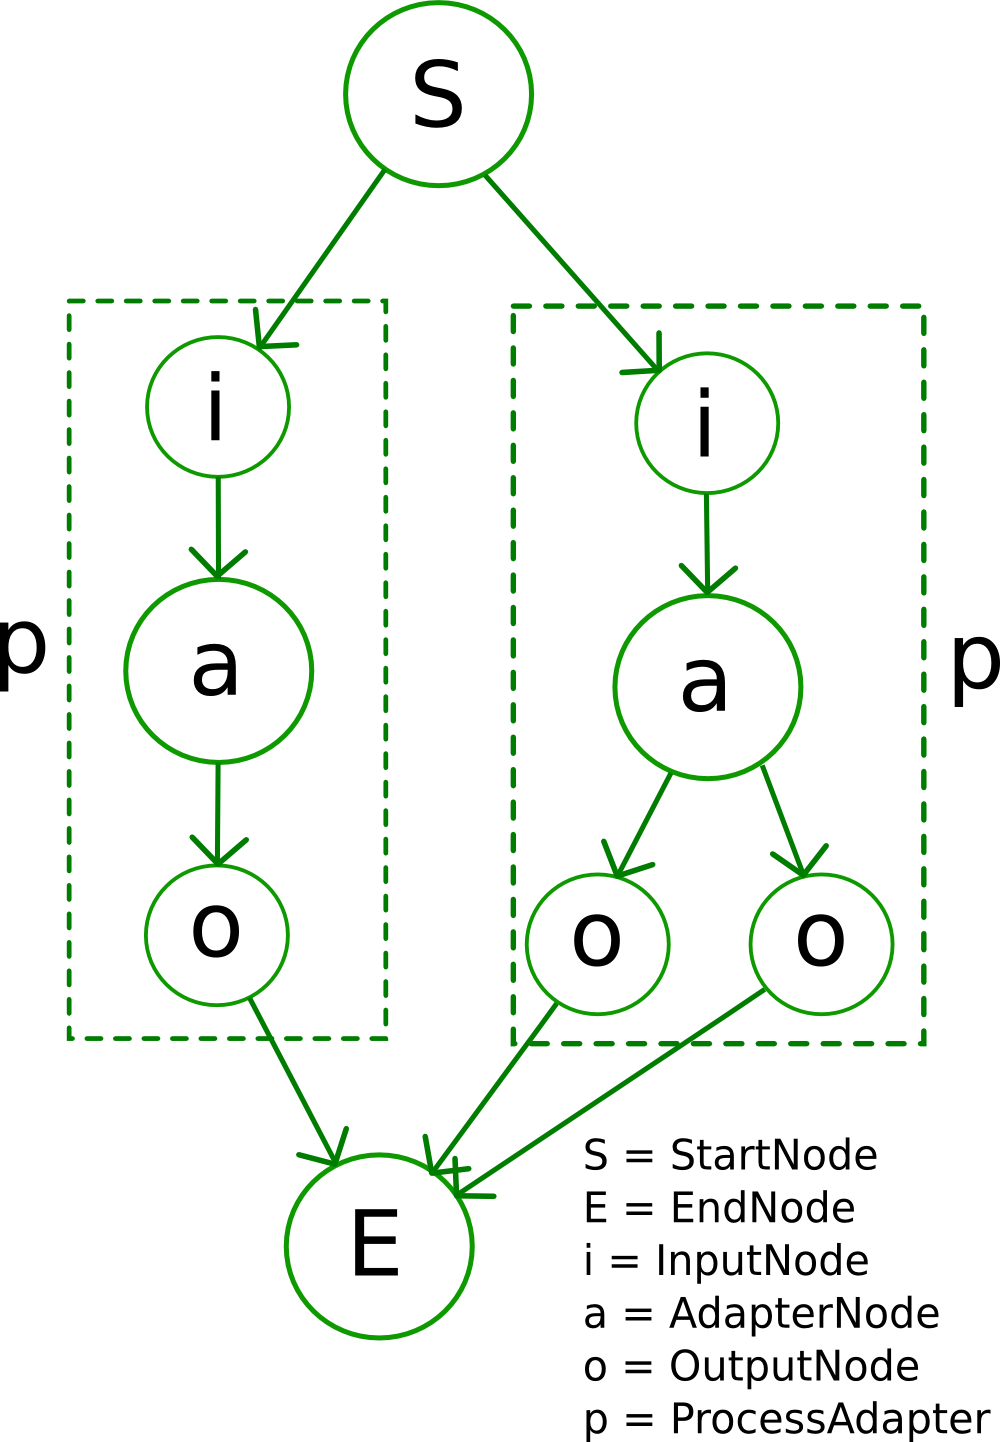
\includegraphics[scale=0.12]{../graphics/graphcomp}
\caption{Beispiel Graph bestehend aus Processing-Klassenobjekten}
\label{graphcomp}
\end{center}
\end{figure}

\subsubsection{Parameter}
Es wäre naheliegend, die Implementation der Parameter und dessen Verbindungsmöglichkeiten, ebenfalls mittels eines Graph-Modells umzusetzen. Es gibt aber, im Gegensatz zum Prozess-Graph, eine entscheidende Vereinfachung: es bestehen keine Abhängigkeiten. Wird ein Parameter verändert, ist es egal in welcher Reihenfolge die verbundenen Nachbarparameter, über die Änderung informiert werden.
So wurde sich für ein einfachen Observer-Entwurf\footnote{im Unterschied zum GoF-Observer, existiert hier jedoch keine Observer Schnittstelle} entschieden (siehe Abbildung \ref{parameterModel}).
\paragraph{ParameterConnection}
Die ParameterConnection-Klasse entspricht dem Observer-Objekt. Jedes Parameter-Objekt enthält eine unbestimmte Menge an ParameterConnection-Objekten. Wird ein Parameterwert verändert, werden diese Objekte benachrichtigt. Zu beachten ist, dass Parameterverbindungen Bidirektional sind. So muss für eine Parameter-Verbindung (A<->B), A sowie B ein ParameterConnection-Objekt (A->B, B->A) enthalten. 

\paragraph{ConnectionOperator}
Neben dem Nachbarparameter enthält ein ParameterConnection-Objekt eine unbestimmte Menge an ConnectionOperatoren. Diese bearbeiten den zu übermittelnden Parameterwert. Auch hier ist die Bidiretionalität zu beachten. Für eine Parameter-Verbindung (A<->B), muss die Verbindung(B->A) die Inverse-Operation zur Verbindung (A->B) enthalten. Den Inverse-ConnectionOperator liefert die Methode: getInverseOperator().
\paragraph{HasParameter}
Die Schnittstelle HasParameter, ermöglicht den zugriff auf eine unbestimmte Menge an Parameterobjekten. So wird diese Schnittstelle, unter anderem, von allen Modulen und den Plugins implementiert. 
\begin{figure}[htbp]
\begin{center}
	\includegraphics[scale=0.45]{../graphics/ParameterOverview}
\caption{Parameter-Klassen Modell}
\label{parameterModel}
\end{center}
\end{figure}
%%%%%%%%%%%%%%%%%%%%%%%%%%%%%%%%%%%%%%%%%%%%%%%%%%%%%%%%%%%%%%%
\subsection{Die GUI Ebene}
\paragraph{PpiEditor}
Die PpiEditor-Klasse implementiert, die von dem Vst-Gui SDK vorgegebene AEffGUIEditor-Klasse. Sie dient der Kommunikation zwischen Hostanwendung und Plugin-Editor.
\paragraph{CView}
Die CView-Klasse ist die Oberklasse aller graphischen Elemente im Vst-Gui SDK. Sie besteht aus einem Rechteckigen Bereich und enthält die Methode draw(CDrawContext *cn). Über diese können mittels übergebenen DrawContext, im sichtbaren Bereich Zeichenoperationen ausgeführt werden.
\paragraph{CircuidView}
Die CircuidView-Klasse repräsentiert die ''Bühne'' der GUI.
Zu beginn der Entwicklung stand der Autor vor der Entscheidung, die Bühnedarstellung nach Vst-Gui SDK Methodik zu gestalten oder eine eigene Implementierung zu verwenden. So könnte jedes Bühnenobjekt einen eigenen CView-Bereich darstellen. Was aus Sicht des Vst-Gui SDKs durchaus logisch wäre, da dort alle graphischen Elemente, wie Regler und Knöpfe, als CView-Klasse implementiert sind. 
\\\\
Es wurde sich allerdings dagegen entschieden. So ist einzig die CircuidView-Klasse eine CView-Klasse. Sie ist für das Zeichnen der Bühne und allen enthaltenen Objekten verantwortlich. Die Gründe für diese Entscheidung waren:
\begin{itemize}
	\item das Vst-Gui SDK wurde nicht für dynamische Oberflächen mit frei beweglichen Objekten entworfen (dargestellt werden üblicherweise Konsolen mit fest positionierten Bedienelementen)
	\item die schlechte Dokumentation des Vst-Gui SDKs (Erschließung hauptsächlich nach ''trial and error'' Prinzip)
	\item weniger direkte Abhängikeiten zum Vst-Gui SDKs (was eine eventuelle Immigration zu einem anderen/besseren Framework erleichtern würde)
\end{itemize}
\paragraph{GObject}
Die GObject-Klasse ist die Oberklasse, aller Objekte die von der CircuidView aufgenommen werden können. Sie bildet das Gegenstück zur PObject Klasse.
\paragraph{GProcessModule}
Die GProcessModule-Klasse ist die graphische Repräsentation der ProcessAdaptor-Objekte.
\paragraph{GIONode}
Die GIONode-Klassen repräsentieren die Input-/OutputNode Objekte.
\paragraph{GConnection}
Die GConnection-Klassen repräsentieren die Verbindungen zwischen den GObjecten.
\paragraph{CViewWrapper}
Wie bereits beschrieben, implementiert die CircuidView-Klasse die Bühnedarstellung, unabhängig von den CView-Klassen. Die CircuidView nimmt ausschließlich GObject-Objekte auf. Dies bedeutet jedoch, dass Vst-Gui SDK Steuerungs-Elemente, nicht mit der CircuidView verwendet werden können. Diesen Nachteil behebt die CViewWrapper-Klasse. Sie hüllt ein CView-Objekt in ein GObject-Objekt. Über ein Template-Parameter wird festgelegt, welche GObject-Klasse Oberklasse ist. Somit ist es möglich, Eine CView-Klasse mit den Eigenschaften von GCircle zu umhüllen.
\begin{figure}[htbp]
\begin{center}
	\includegraphics[scale=0.45]{../graphics/gui_overview}
\caption{Parameter-Klassen Modell}
\label{parameterModel}
\end{center}
\end{figure}
%%%%%%%%%%%%%%%%%%%%%%%%%%%%%%%%%%%%%%%%%%%%%%%%%%%%%%%%%%%%%%%
\subsection{Die Control Ebene}
\paragraph{CircuidControl}
\paragraph{FrontController}
%gründe für mvc
% !TEX encoding = UTF-8 Unicode
\section{Realisierung}
\subsection{SDK Probleme}
%string längen
%Parameter::setValue( VstNumber v ) avoid NaN. problems with serialize and deserialize issue #113
%midi receive
%getLocation
%fruity
%Cant add vst-directories in VSTForx configuration dialog
Da VSTForx sowohl ein Plugin, als auch ein Host für Plugins ist, existieren gleich zwei potentielle Fehlerquellen. Zum einen muss sichergestellt werden, dass jede Host-Anwendung VSTForx Laden und Ausführen kann. Zum anderen sollte auch VSTForx in der Lage sein, jedes Plugin zu Laden und Auszuführen. Unglücklicherweise ist eine große schwäche des VST2.x-SKDs, die schlechte Dokumentation. So sind viele Funktionen ungenügend oder gar nicht beschrieben. Auch bleibt ungeklärt, in welcher Reihenfolge Operationen ausgeführt werden(siehe Abschnitt: Initalisierungsreihenfolge). Da es eine große Menge an Plugins und Host-Anwendungen gibt, führte dies zu einer Reihe an Problemen, die erst durch viel ausprobieren ermittelt und behoben werden konnten. 
\paragraph{Initalisierungsreihenfolge}
Wie bereits in Kapitel \ref{kapAnforderungen} beschrieben, existiert zur Kommunikation zwischen Host und Plugin lediglich eine Methode: \funktion{dispatcher()}.

// reihenfolge wichtig! ( ueber debugger ermittelt )
// setze samplerate  
plug.aEff->dispatcher ( plug.aEff, effSetSampleRate, 0, 0, 0, plug.hostInfo->getSampleRate() );
// setze blockSize  
plug.aEff->dispatcher ( plug.aEff, effSetBlockSize, 0, plug.hostInfo->getBlockSize(), 0, 0 );
// open
plug.aEff->dispatcher ( plug.aEff, effOpen, 0, 0, 0, 0.0 );
aEff->dispatcher ( aEff, effMainsChanged, 0, 1, 0, 0 ); // turn on
aEff->dispatcher ( aEff, effMainsChanged, 0, 0, 0, 0 ); // turn off
aEff->dispatcher ( aEff, effMainsChanged, 0, 1, 0, 0 ); // turn on


\paragraph{String längen}
\paragraph{NaN Probleme}
\paragraph{Kein Midi-Empfang}
\paragraph{Wo bin ich?}
\paragraph{Verzeichnisauswahl}

%%%%%%%%%%%%%%%%%%%%%%%%%%%%%%%%%%%%%%%%%%%%%%%%%%%%%%%%%%%%%%%%%%%%
\subsection{Persistenz}
%Serialisierungs problem : ein prozess
%%%%%%%%%%%%%%%%%%%%%%%%%%%%%%%%%%%%%%%%%%%%%%%%%%%%%%%%%%%%%%%%%%%%
\subsection{Die Plugindatenbank}
\paragraph{Testen}
\paragraph{Probleme}
%%%%%%%%%%%%%%%%%%%%%%%%%%%%%%%%%%%%%%%%%%%%%%%%%%%%%%%%%%%%%%%%%%%%
\subsection{Die Benutzerschnitstelle}
\paragraph{Probleme}

%\include{kap_Bedienungsanleitung}
%% !TEX encoding = UTF-8 Unicode
\section{Fazit}
Mit \emph{C++} als Entwicklungssprache wurde eine mächtige und performante, aber auch fehleranfällige und unsicherere Programmiersprache gewählt. Einerseits wurden die in ''modernen'' Programmiersprachen eher unspektakulären Aufgaben, wie das Einbinden einer externen Bibliothek, als besonders zeitaufwändig empfunden (fehlendes Paketmanagment). Andererseits wird der Entwickler gerade durch solche Fallstricke zu mehr Sorgfalt gezwungen, und das allgemeine Verständnis für Programmiersprachen erhöht. 
Insbesondere wurde die Boost-Bibliothek schätzen gelernt, welche \emph{C++} um ''moderne'' Programmiertechniken wie den 'Smart Pointer' erweitert. 
\\\\
Mit VSTForx ist es - nach Meinung des Autors - gelungen, ein interessantes und spanendes Werkzeug zu entwickeln. Dennoch ist die Entwicklung an VSTForx noch nicht abgeschlossen. Folgend werden zukünftige (mögliche) Verbesserungen oder Erweiterungen besprochen. 
\subsection{Verbesserungen}
\subsubsection{GUI}
Die VST-GUI Bibliothek bietet leider zu wenig oder unzureichend implementierte Funktionen, um eine vollwertige GUI-Anwendung zu entwickeln. So sind die meisten Elemente in VST-GUI, bitmapbasierend und mit festen Positionen versehen. Eine Schaltfläche muss daher erst gezeichnet und dann platziert werden. Eine dynamische Anwendung (Objekte veränderbar in Größe und Position) mit einheitlichem Look-And-Feel, kann somit nur sehr schwer umgesetzt werden. 
\\\\
Wünschenswert wäre hier die Verwendung eines GUI-Toolkits, wie \emph{Qt\footnote{http://qt.nokia.com}} oder \emph{WxWidgets\footnote{http://www.wxwidgets.org}}. Leider konnte  noch kein passendes Toolkit gefunden werden. Jedes (bisher geprüfte) Toolkit erzeugt und verwaltet ein eigenes Fenster, um darin Objekte zu platzieren. VST-Plugins verwenden allerdings ein von der Hostanwendug (teilweise mit eigener Dekoration) erzeugtes Fenster. Es muss daher ein Toolkit gefunden (oder entwickelt) werden, welches basierend auf einen bereits existierenden ''Window-Handler'', GUI-Funktionen bietet.
\\\\
Im Falle einer Eigenentwicklung käme die \emph{Cairo\footnote{http://cairographics.org/}}-Bibliothek in Frage. Diese bietet sehr leistungsfähige Zeichenfunktionen und ist, wie gefordert, in bestehende Fensterumgebungen einbindbar.
\subsubsection{'Signal nach Parameterwert'-Problem}
'Signal nach Parameterwert'-Module, welche ein Eingangsignal analysieren, um einen Parameterwert zu steuern, haben eine Einschränkung: Sie werden, da sie als \emph{ProcessAdapter} in den Graph eingebunden sind, nur einmal pro Sampleblock ausgeführt. Das bedeutet, dass ein Parameterwert sich immer seltener ändert, je höher die Sampleblockgröße ist. Bei einer Samplerate von 44100.0Hz und einer (üblichen) Blockgröße von 1024 wird demnach ein Parameter alle 23Ms aktualisiert. Dies ist vermutlich kaum wahrnehmbar, nach Meinung des Autors dennoch ein kleiner Schönheitsfehler.
\\\\
Zur Lösung müsste die Parameter-Aktualisierung entsprechender Module in einem separaten Thread mit fester Aktualisierungsrate durchgeführt werden. 
\subsubsection{Weitere Module}
\paragraph{'Frequenz nach Wert'-Modul}
Denkbar wäre ein 'Signal nach Parameterwert'-Modul, welches die Grundtonfrequenz eines Signals ermittelt und als Parameterwert ausgibt. In einem früheren Projekt wurde ähnliches mittels FFT-Analyse bereits realisiert. Der Algorithmus - welcher in der Sprache C vorliegt - müsste angepasst und als \emph{ProcessAdapter} eingebunden werden.  
\paragraph{Skript-Unterstützung}
Da die Entwicklung zusätzlicher Module viel Arbeit und Zeit in Anspruch nimmt (Implementierung verschiedener Klassen, lange Kompilierungszeiten), wäre es hilfreich, mittels einer dynamischen Skriptsprache Module zu entwerfen, ohne das eigentliche Programm neu kompilieren zu müssen. 
\\\\
So wäre ein Modultyp denkbar, der seine Berechnungszeit an ein externes Skript weitereichen würde. Besonders geeignet wäre hierfür die Skriptsprache \emph{Lua\footnote{http://www.lua.org/}}. Lua ist kompiliert nur wenige Kilobyte groß und sehr leicht in ein bestehendes C/C++ - Programm einbindbar. 
Auf ähnlichem Wege wären auch benutzerdefinierte Parameter-Operatoren denkbar.

 
% !TEX encoding = UTF-8 Unicode
\section{Literaturverzeichnis}
% !TEX encoding = UTF-8 Unicode
\begin{thebibliography}{-------}
%##########################################################
	\bibitem[STEIN01]{Stein01}
		Steinberg Media Technologies GmbH:
		{\em Steinberg releases VST 2.4 standard with new features},
		http://www.steinberg.net/index.php?id=334\&L=1, Aufgerufen am 13.12.2011
%##########################################################
	\bibitem[STEIN02]{Stein02}
		Steinberg Media Technologies GmbH:
		{\em Steinberg releases VST3 SDK},
		http://www.steinberg.net/en/company/press/archive/2008/steinberg\_vst3\_sdk.html, Aufgerufen am 13.12.2011
%##########################################################
	\bibitem[VST]{Vst}
		Steinberg Media Technologies GmbH:
		{\em Steinberg VST SDK 2.4 Documentation}, 2006
%##########################################################
	\bibitem[KARK]{Karkos}
		Konrad Karkos: \emph{Digitale Musikproduktion}, MAGIX AG 2010
%##########################################################
	\bibitem[GOER]{Goerne}
		Thomas Görne: \emph{Tontechnik}, Carl Hanser Verlag 2008
%##########################################################
	\bibitem[REAK]{Reaktor}
		Native Instruments GmbH:
		{\em Reaktor Core Technology},
		http://www.native-instruments.com/\#/de/products/producer/reaktor-55/?page=1626, Aufgerufen am 1.02.2012
%##########################################################
	\bibitem[ABL]{Ableton}
		Dennis DeSantis: \emph{Ableton Benutzerhandbuch Version 8}, Ableton AG 2010
%##########################################################
	\bibitem[BGL]{Bgl}
		Jeremy G.Siek: \emph{The Boost Graph Library}, Addison-Wesely 2001
%##########################################################
	\bibitem[GOF]{Gof}
		Erich Gamma: \emph{Entwurfsmuster}, Addison-Wesely 2009
%##########################################################
	\bibitem[TAN]{Tan}
         Andrew S. Tanenbaum: \emph{Moderne Betriebssysteme}, Pearson Education 2009
%##########################################################
	\bibitem[STEP]{Stephens}
		D. Ryan Stephens: \emph{C++ Cookbook}, O'Reilly 2005
%##########################################################
	\bibitem[RED]{Reddy}
		Martin Reddy: \emph{API Design for C++}, Academic Press 2011
\end{thebibliography}


% !TEX encoding = UTF-8 Unicode
\section{Abbildungs Verzeichnis}
\listoffigures
%\include{kap_Index}
%% !TEX encoding = UTF-8 Unicode
\section{Quelltextverzeichnis}
\lstlistoflistings

\end{document}